\let\negmedspace\undefined
\let\negthickspace\undefined
\documentclass[journal]{IEEEtran}
\usepackage[a5paper, margin=10mm, onecolumn]{geometry}
%\usepackage{lmodern} % Ensure lmodern is loaded for pdflatex
\usepackage{tfrupee} % Include tfrupee package

\setlength{\headheight}{1cm} % Set the height of the header box
\setlength{\headsep}{0mm}     % Set the distance between the header box and the top of the text

\usepackage{gvv-book}
\usepackage{gvv}
\usepackage{cite}
\usepackage{amsmath,amssymb,amsfonts,amsthm}
\usepackage{algorithmic}
\usepackage{graphicx}
\usepackage{textcomp}
\usepackage{xcolor}
\usepackage{txfonts}
\usepackage{listings}
\usepackage{enumitem}
\usepackage{mathtools}
\usepackage{gensymb}
\usepackage{comment}
\usepackage[breaklinks=true]{hyperref}
\usepackage{tkz-euclide} 
\usepackage{listings}
\usepackage{gvv}                                        
\def\inputGnumericTable{}                                 
\usepackage[latin1]{inputenc}                                
\usepackage{color}                                            
\usepackage{array}                                            
\usepackage{longtable}                                       
\usepackage{calc}                                             
\usepackage{multirow}                                         
\usepackage{hhline}                                           
\usepackage{ifthen}                                           
\usepackage{lscape}
\usepackage{circuitikz}
\tikzstyle{block} = [rectangle, draw, fill=blue!20, 
    text width=4em, text centered, rounded corners, minimum height=3em]
\tikzstyle{sum} = [draw, fill=blue!10, circle, minimum size=1cm, node distance=1.5cm]
\tikzstyle{input} = [coordinate]
\tikzstyle{output} = [coordinate]

\begin{document}


\bibliographystyle{IEEEtran}
\vspace{3cm}

\title{4.7.46}
\author{EE25BTECH11049 - Sai Krishna Bakki}
 \maketitle
% \newpage
% \bigskip
{\let\newpage\relax\maketitle}

\renewcommand{\thefigure}{\theenumi}
\renewcommand{\thetable}{\theenumi}
\setlength{\intextsep}{10pt} % Space between text and floats


\numberwithin{equation}{enumi}
\numberwithin{figure}{enumi}
\renewcommand{\thetable}{\theenumi}
\textbf{Question:}\\
The equations of the lines passing through the point (1, 0) and at a distance $\frac{\sqrt{3}}{2}$ from the origin, are \\

\solution
\subsection*{1. Represent the Line with Matrices}

We can represent the equation of a line in its normal form using matrix notation:
\begin{align}
\vec{n}^T \vec{x} - p = 0
\end{align} 
Where:
\begin{itemize}
    \item $\vec{n}$ is the \textbf{unit normal vector} to the line. \begin{align}\vec{n} = \myvec{\cos\theta \\ \sin\theta}\end{align} 
    \item $\vec{x}$ is a vector to any point $(x, y)$ on the line. \begin{align}\vec{x} = \myvec{x \\ y}\end{align} 
    \item $p$ is the perpendicular distance from the origin to the line.
\end{itemize}
From the problem, we are given:
\begin{itemize}
    \item The distance from the origin, \begin{align}p = \frac{\sqrt{3}}{2}\end{align} 
    \item A point on the line, $(1, 0)$, which we can represent as a vector \begin{align}\vec{p_1} = \myvec{1 \\ 0}\end{align} 
\end{itemize}

\subsection*{2. Formulate and Solve the Matrix Equation}

Since the point $\vec{p_1}$ lies on the line, it must satisfy the line's equation:
\begin{align}\vec{n}^T \vec{p_1} - p = 0\end{align}
Now, we substitute the known matrices and scalars into this equation:
\begin{align}
\myvec {\cos\theta & \sin\theta } \myvec{1 \\ 0} - \frac{\sqrt{3}}{2} = 0 \end{align}
Performing the matrix multiplication gives a scalar equation:
\begin{align}
\cos\theta &= \frac{\sqrt{3}}{2}
\end{align}

\subsection*{3. Determine the Normal Vectors}

Using the identity,
\begin{align}
    \myvec{\cos\theta & \sin\theta}\myvec{\cos\theta \\ \sin\theta}=1
\end{align}
 we can find the possible values for $\sin\theta$:
\begin{align}
\myvec{\frac{\sqrt{3}}{2} & \sin\theta}\myvec{\frac{\sqrt{3}}{2} \\ \sin\theta}=1\\
\sin^2\theta = \frac{1}{4} &\implies \sin\theta = \pm \frac{1}{2}
\end{align}
This gives us two possible unit normal vectors for our two lines:
\begin{align}
\vec{n_1} = \myvec{\frac{\sqrt{3}}{2} \\ \frac{1}{2}}\\
\vec{n_2} = \myvec{\frac{\sqrt{3}}{2} \\ -\frac{1}{2}}
\end{align}
\subsection*{4. Find the Equations of the Lines}

We can now find the equation for each line by substituting its normal vector back into the general matrix equation $\vec{n}^T \vec{x} - p = 0$.

\textbf{Line 1:} Using $\vec{n_1}$
\begin{align}
\myvec{ \frac{\sqrt{3}}{2} & \frac{1}{2}} \myvec{x \\ y} - \frac{\sqrt{3}}{2} = 0 
\end{align}
Multiplying by 2, we get the first equation:
\begin{align}
 \myvec{\sqrt{3}&1}\vec{x}=\sqrt{3} 
 \end{align}

\textbf{Line 2:} Using $\vec{n_2}$
\begin{align}
\myvec{\frac{\sqrt{3}}{2} & -\frac{1}{2}} \myvec{x \\ y} - \frac{\sqrt{3}}{2} = 0
\end{align}
Multiplying by 2, we get the second equation:
\begin{align}   
 \myvec{\sqrt{3}&-1}\vec{x}=\sqrt{3} 
\end{align}
The equations of the lines passing through the point (1, 0) and at a distance $\frac{\sqrt{3}}{2}$ from the origin, are 
\begin{align}
     \myvec{\sqrt{3}&-1}\vec{x}=\sqrt{3} ,\myvec{\sqrt{3}&1}\vec{x}=\sqrt{3}
\end{align}
\newpage
 \begin{figure}
    \centering
    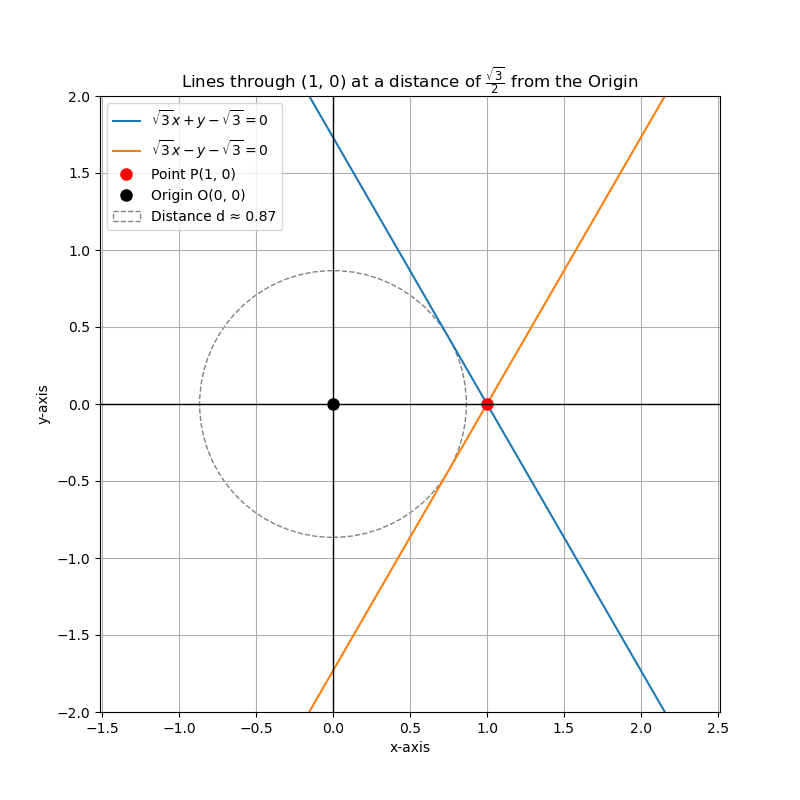
\includegraphics[width=0.9\columnwidth]{figs/Figure_1.png}
    \label{fig:placeholder}
    \caption{}
\end{figure}
\end{document}